\subsection{Recorridos funcionales y evidencia}

La revisión del prototipo describe las vistas de la aplicación desarrollada y los recorridos previstos: localizar una hospitalización autorizada, consultar información externa y notas propias, redactar o dictar una nota, revisar transcripción y asistencia de redacción, confirmar la nota y solicitar un resumen del período seleccionado. Esta descripción de la implementación no equivale a una prueba observada con participantes ni demuestra usabilidad, eficacia, seguridad, calidad, latencia o aceptación.

Los recorridos enlazan la consulta de la FCE con el registro de contexto y la asistencia local. La revisión distingue el contenido obtenido de la fuente, las notas confirmadas por su autor y los resúmenes derivados para consulta. La evidencia y las condiciones de evaluación de estos recorridos se documentan en la sección de verificación y validación.

La evidencia visual combina las cinco maquetas históricas de la sección de fabricación preliminar, que representan diseño, con una selección de capturas de la interfaz implementada. Las capturas documentan pantallas, no prueban por sí solas autorización, operación local efectiva de modelos ni calidad funcional. No se han realizado pruebas con participantes ni en producción. La demostración se limita a información sintética y no acredita aptitud para datos clínicos reales, integración productiva con una institución, seguridad hospitalaria productiva ni cumplimiento normativo garantizado.

La selección sigue algunos recorridos de la interfaz; las maquetas históricas se conservan en la sección de fabricación preliminar y no deben confundirse con estas capturas de implementación.

\subsubsection*{Acceso y consulta de hospitalizaciones}

La Figura~\ref{fig:impl-acceso} reúne las pantallas de autenticación y listado de hospitalizaciones.

\begin{figure}[H]
    \centering
    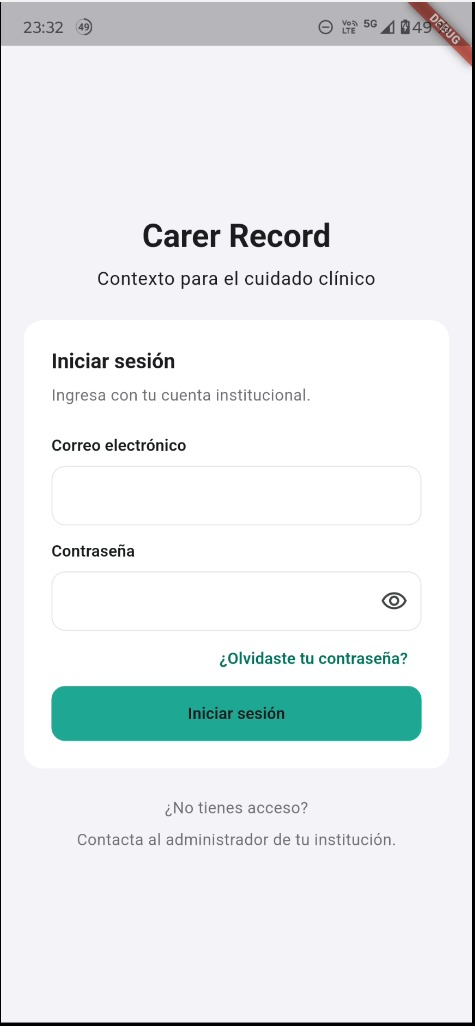
\includegraphics[width=0.45\textwidth]{Imagenes/app_autenticacion.jpeg}
    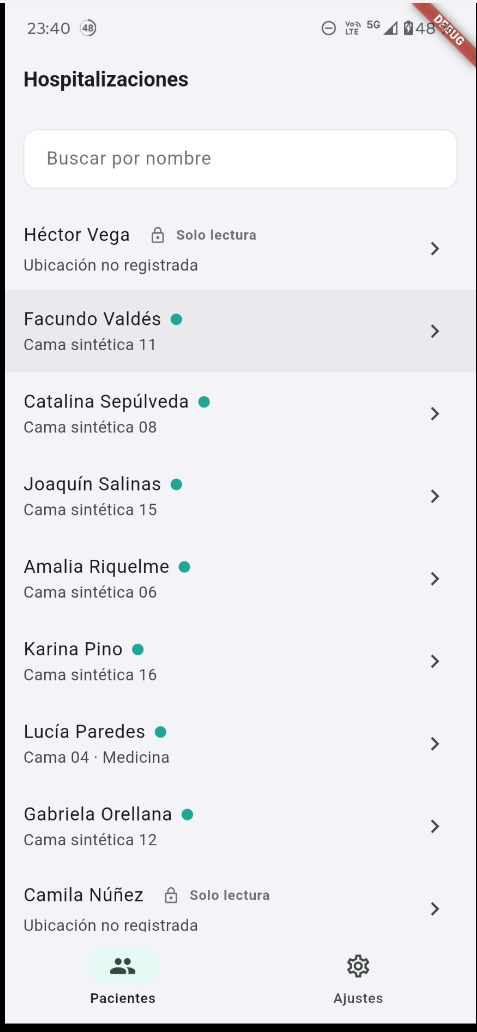
\includegraphics[width=0.45\textwidth]{Imagenes/app_hospitalizaciones.jpeg}
    \caption{Interfaz implementada: autenticación y hospitalizaciones (datos sintéticos).}
    \label{fig:impl-acceso}
\end{figure}

\subsubsection*{Consulta clínica y registro de contexto}

La Figura~\ref{fig:impl-ficha} reúne vistas de la ficha clínica. La Figura~\ref{fig:impl-nota} muestra la revisión de una nota dictada y su aparición en la bitácora.

\begin{figure}[H]
    \centering
    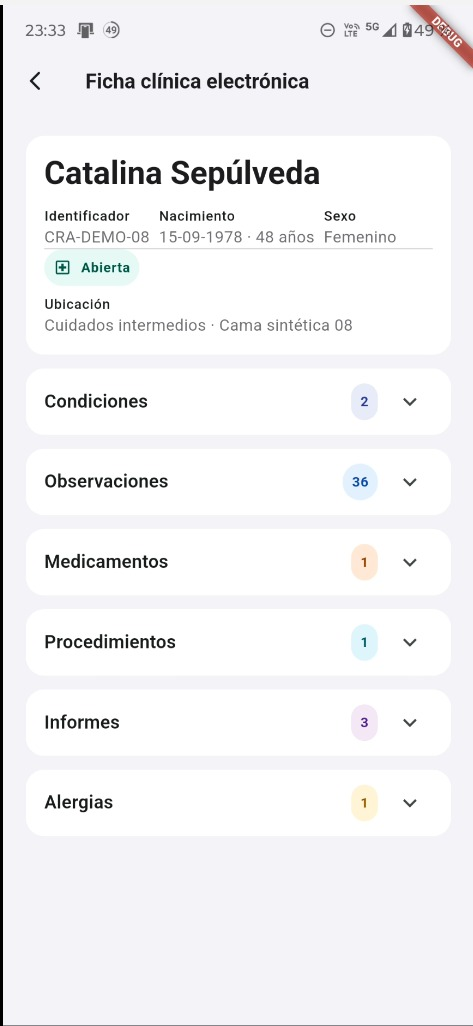
\includegraphics[width=0.45\textwidth]{Imagenes/app_ficha_clinica_general.jpeg}
    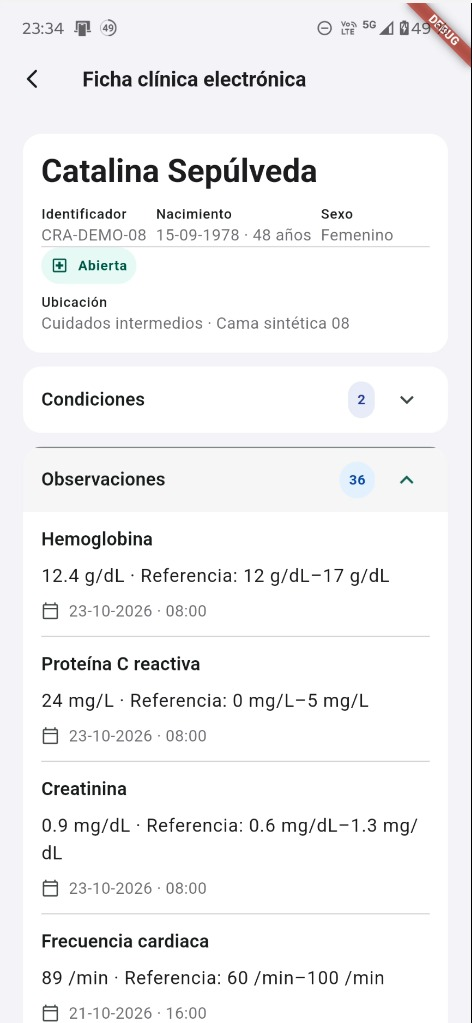
\includegraphics[width=0.45\textwidth]{Imagenes/app_ficha_clinica_observaciones.jpeg}
    \caption{Interfaz implementada: vistas de ficha clínica (datos sintéticos).}
    \label{fig:impl-ficha}
\end{figure}

\begin{figure}[H]
    \centering
    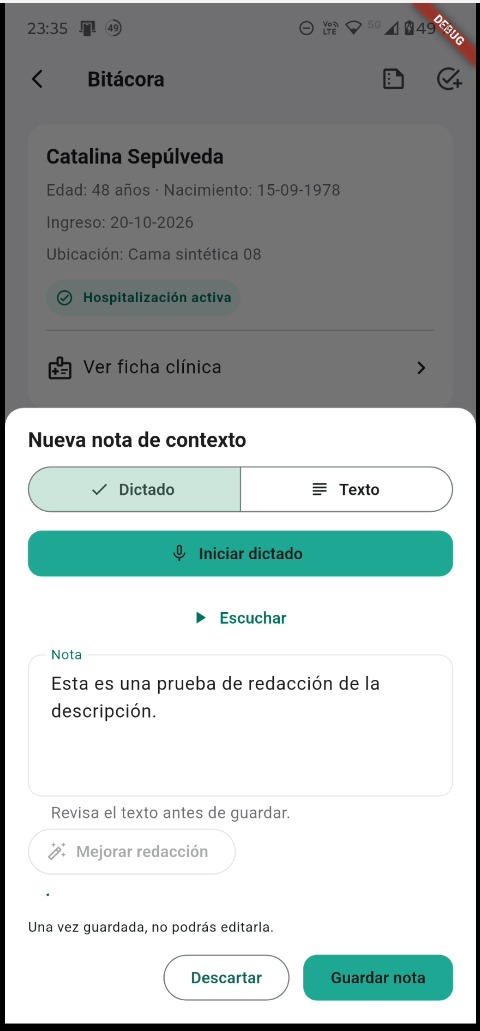
\includegraphics[width=0.45\textwidth]{Imagenes/app_nota_dictada_revision.jpeg}
    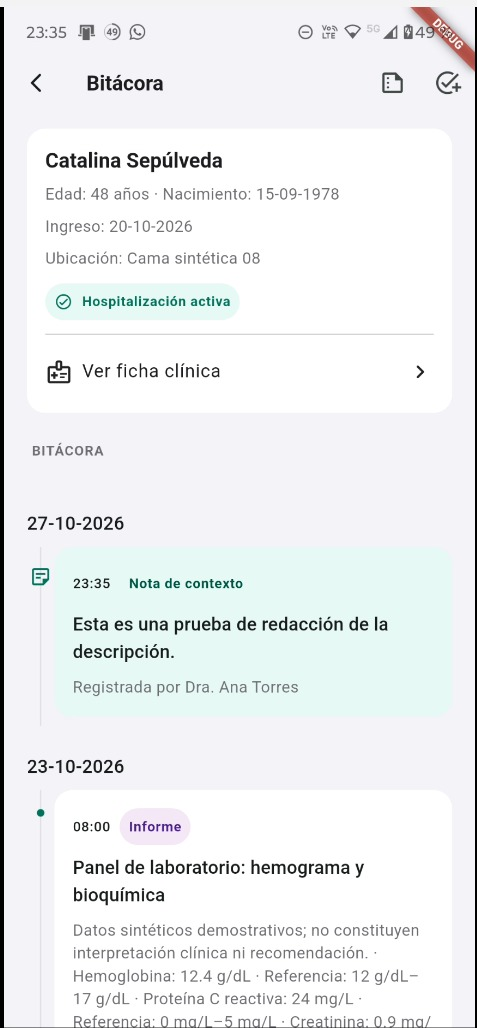
\includegraphics[width=0.45\textwidth]{Imagenes/app_bitacora_nota_confirmada.jpeg}
    \caption{Interfaz implementada: revisión de nota dictada y bitácora (datos sintéticos).}
    \label{fig:impl-nota}
\end{figure}

\subsubsection*{Configuración visible}

La Figura~\ref{fig:impl-configuracion} muestra la interfaz de configuración de permisos clínicos y la pantalla de modelos locales; no constituye evidencia de autorización efectiva ni de procesamiento local efectivo.

\begin{figure}[H]
    \centering
    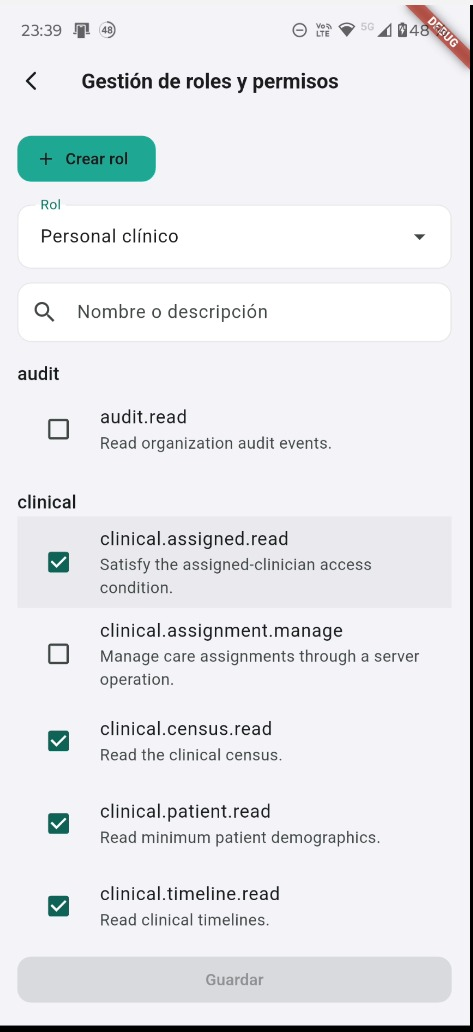
\includegraphics[width=0.45\textwidth]{Imagenes/app_roles_permisos_clinicos.jpeg}
    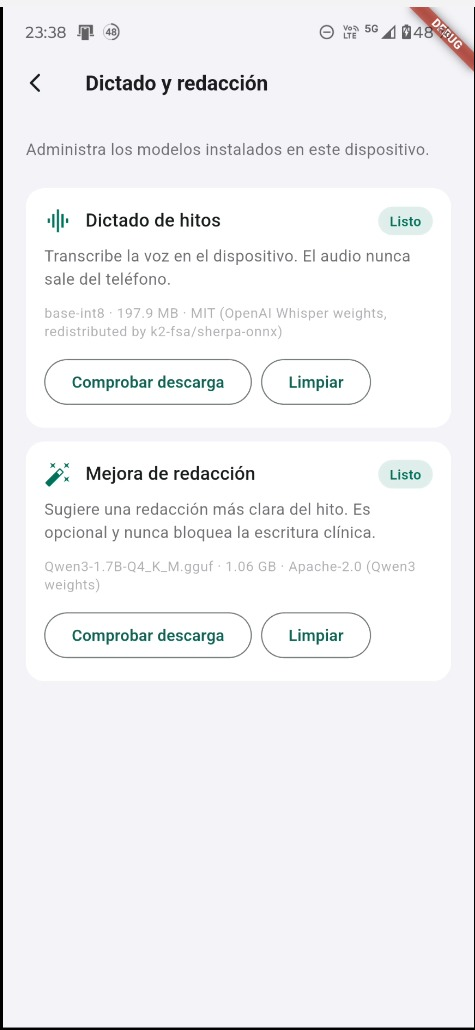
\includegraphics[width=0.45\textwidth]{Imagenes/app_modelos_locales.jpeg}
    \caption{Interfaz implementada: permisos clínicos y modelos locales (datos sintéticos).}
    \label{fig:impl-configuracion}
\end{figure}
